Vor der Implementierungsphase wurden die vorherrschenden Gegebeneiten sowie der angestrebte Soll-Zustand analysiert und   Kalkulationen betreffend der Implementierungskosten durchgeführt.

\subsection{Projektschnittstellen}
    Die Projektschnittstellen können in Personen- und technische Schnittstellen unterteilt werden. In diesem Rahmen wirkte die Fachbetreuerin, Frau Bitterlich, bei der Projektplanung und Anforderungsausarbeitung sowie in nachträglichen Absprachen zum Projekt mit. Unterstützung während der Entwicklung und zur Code Review wurde durch Herrn Schilde, Herrn Schubert und Herrn Makarov gestellt. Anwendertests wurden durch Mitarbeiter der Abteilung Human Resources durchgeführt.\\
    Technische Schnittstellen sind die relationalen Datenbanken des Unternehmens sowie der Relaunch der unternehmenseigenene Administration.

\subsection{Ist-Analyse}
    Die derzeit produktiv genutzte Unternehmens-Administration (im Folgenden \glqq die Admin\grqq{}) basiert backendseitig technisch auf Perl mit dem Framework \glqq Catalyst\grqq{}, welches ergänzt wird durch das hauseigen entwickelte und ebenfalls darauf aufbauende Framework \glqq Mariposa\grqq{}. \mbox{Dieses} stellt die jeweiligen Tools nach dem MVC-Design Pattern\footnote{Model View Controller} bereit. Das HTML der Anwendung wird weitestgehend serverseitig mit Hilfe der Template Engine \glqq Template Toolkit\grqq{} gerendert. Für clientseitige Veränderungen der angezeigten Web-Anwendung kommt JavaScript und jQuery zum Einsatz.\\
    Eines der bereitgestellten Tools ist das Kontakt-Tool, über welches die Mitarbeiter des Unternehmens gesucht und unter anderem die Kontaktdaten angezeigt werden können. Die Fachabteilung Human Resources kann über dieses Tool auch weiterführende Informationen, wie den Urlaubsanspruch oder Fehlgründe, für einzelne Mitarbeiter abrufen. Diese sogenannten Stammdaten werden momentan doppelt gepflegt - ein Mal in einer MySQL Datenbank und zusätzlich über das im Unternehmen genutzte Zeiterfassungssystem der Tempras AG. Die \mbox{Pflege} soll zukünftig ausschließlich über das Zeiterfassungssystem erfolgen. Anschließend \mbox{sollen} die Datensätze in der Datenbank aus diesem Bestand aktualisiert werden.\\

    \subsection{Soll-Analyse}
    Um die Admin zu modernisieren, wurde sich dazu entschieden, das bestehende System nicht zu überholen, sondern dieses zu relaunchen. Dadurch wird nicht nur die Codebasis entschlackt, auch die insgesamte Performance der Admin steigt durch den damit einhergehenden Sprachwechsel sowohl auf PHP mit dem Framework \glqq Laravel\grqq{} als auch auf Node.js zum Bereitstellen serverseitig vorgerenderter Webseiten. Das JavaScript-Framework \glqq React\grqq{} übernimmt das \mbox{clientseitige} Rendern der Web-App. Die Anwendung folgt somit weiterhin dem MVC-Prinzip.\\
    Das neue Kontakt-Tool soll, im Gegensatz zum alten, auch keine Spreadpartner, sondern nur noch Angestellte anzeigen und zum Zeitpunkt der Abgabe technisch soweit vorbereitet sein, dass ein späteres Hinzufügen eines Rollen- und Rechtesystems möglichst einfach umzusetzen ist. Die sonstige Usability soll im Vergleich zur alten Kontaktsuche weitestgehend erhalten bleiben.

    \begin{figure}[h]
        \centering
        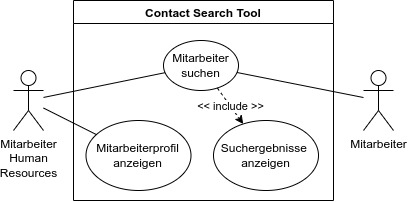
\includegraphics[width=0.75\textwidth]{suche_use-case.jpg}
        \caption{Anwendungsfalldiagramm \glqq Kontaktsuche\grqq{}}
    \end{figure}

\subsection{Make-Or-Buy Analyse}
    Die Option, eine externe Software für diesen Anwendungsfall einzukaufen, wurde schnell verworfen, da die Vorteile einer Eigenentwicklung überwiegen. Ein fremdentwickeltes Produkt bringt beispielsweise mit, dass zusätzliche Schnittstellen zum restlichen System geschaffen werden müssten und die Software entweder in einer gesonderten Form in den Admin Relaunch eingebettet werden müsste, was zusätzliche Kosten verursachen würde, oder als Standalone Anwendung betrieben wird, wodurch der Gedanke einer zentralen Tool-Sammlung nicht konsequent umgesetzt wird.\\
    Eine interne Entwicklung des Kontakt-Tools hat mehrere hervorzuhebende Vorteile. Zum einen ist das zugrundeliegende System mit seinen Schnittstellen bekannt. Zum anderen kann die Software von Anfang an in die Codebasis des Admin Relaunch integriert und punktgenau auf die Anforderungen der Fachabteilung zugeschnitten werden. Auch die spätere Wartung ist einfacher zu realisieren, da dies durch die IT-Entwicklungsabteilung erfolgen kann und kein Bedarf an Wartungsverträgen vorliegt, der ebenfalls wieder Kosten verursacht. Hinzu kommt, dass im Unternehmen vorhandene Technologien wie React, Node.js, CSS, PHP und MySQL genutzt werden und dadurch bereits ausreichend Know-How vorhanden ist, um eine kompetente Wartung zu gewährleisten. Insofern sind die Kosten einer Eigenentwicklung tendenziell geringer als der Kauf eines externen Produktes.\\


\vfill
\pagebreak

\subsection{Kostenanalyse}
    Für die Kostenanalyse werden Personal- und Betriebskosten zur Software-Entwicklung im Rahmen des Projektes in Betracht gezogen. Zur Berechnung der Personalkosten wurden Bruttogehälter in Höhe von monatlich 1.350\,€ für Auszubildende, 1.900 € für Mitarbeiter der Fachabteilung Human Resources und 2.500\,€ für Entwickler veranschlagt. Des Weiteren wurde eine tägliche Arbeitszeit von 8 Stunden je Mitarbeiter und monatlich durchschnittlich 21 Arbeitstage veranschlagt.\\
    Je Arbeitsplatz wurden pauschal 20\,€ Betriebskosten pro Tag veranschlagt. Darin sind Kosten für vorhandene Soft- und Hardware sowie Strom- und Heizkosten beinhaltet.\\
    Aus diesen Eckdaten ergibt sich ein Stundensatz von 10,54\,€ für den Auszubildenden, 13,81\,€ pro Human Resources Mitarbeiter und 17,38\,€ pro Software-Entwickler.\\
    Der Auszubildende hat insgesamt 120 Mannstunden für das Projekt aufgewendet. Hinzu kommen insgesamt 8 Mannstunden, die Mitarbeiter der Software-Entwicklung in betreuender Form und für Tests aufgewendet haben und 4 Stunden eines Mitarbeiters von Human Resources, der ebenfalls ausführliche Anwendertests durchgeführt und an Projektmeetings teilgenommen hat. Dadurch ergeben sich Gesamtkosten von 1423,80\,€.\\
    Eine detaillierte Kostenrechnung ist in \hyperref[anlage:kosten]{Anlage C} zu finden.

